%===============
%一行目に必ず必要
%文章の形式を定義
%===============
\documentclass{ujarticle}
%===============
%パッケージの定義、必要か不明
%===============
%この下4つを加えることで、mathbbが機能した
\usepackage{amsthm}
\usepackage{amsmath}
\usepackage{amssymb}
\usepackage{amsfonts}
\usepackage{my-default}
%リンク用パッケージ
\usepackage[dvipdfmx]{hyperref}
%tikz用パッケージ
\usepackage[dvipdfmx]{graphicx}
\usepackage{tikz}
\usepackage{tikz-cd}
\usepackage{my-default}

%複数行コメント
%\usepackage{comment}

%修論当時
\newcommand\X{\mathfrak{X}}
\newcommand\p{\mathfrak{p}}
\newcommand\f{\mathfrak{f}}
\newcommand\m{\mathfrak{m}}
\newcommand\G{\mathrm{Gal}}
\newcommand\iy{\infty}
\def\F{F_{\infty}}
\def\M{M_{\infty}}
\def\bgn{\begin}
\def\c{c_{F_{\iy}/M_{\iy}}}
\def\n{\nu_{F_{\iy}/M_{\iy}}}

\newcommand\bqy{\bgn{end{equation*}array*}}
\newcommand\eqy{\end{end{equation*}array*}}
\newcommand\mac{\mathcal}
\newcommand\mf{\mathfrak}
\newcommand\mr{\mathrm}
\newcommand\mb{\mathbb}

\newcommand\vp{\varprojlim}
\newcommand\ot{\otimes}


\renewenvironment{itemize}%
{%
   \begin{list}{\parbox{1zw}{$\bullet$}}% 見出し記号/直後の空白を調節
   {%
      \setlength{\topsep}{0zh}
      \setlength{\itemindent}{0zw}
      \setlength{\leftmargin}{2zw}%  左のインデント
      \setlength{\rightmargin}{0zw}% 右のインデント
      \setlength{\labelsep}{1zw}%    黒丸と説明文の間
      \setlength{\labelwidth}{3zw}%  ラベルの幅
      \setlength{\itemsep}{0em}%     項目ごとの改行幅
      \setlength{\parsep}{0em}%      段落での改行幅
      \setlength{\listparindent}{0zw}% 段落での一字下り
   }
}{%
   \end{list}%
}


\renewenvironment{enumerate}
{
\begin{list}{(\arabic{enumi})}
{
\usecounter{enumi}
\setlength{\topsep}{0zh}
\setlength{\itemindent}{0zw}
\setlength{\leftmargin}{2zw} % 左のインデント
\setlength{\rightmargin}{0zw} % 右のインデント
\setlength{\labelsep}{1zw} % 黒丸と説明文の間
\setlength{\labelwidth}{3zw} % ラベルの幅
\setlength{\itemsep}{0em} % 項目ごとの改行幅
\setlength{\parsep}{0em} % 段落での改行幅
\setlength{\listparindent}{1zw} % 段落での一字下り
}
}{
\end{list}
}



%タイトルデータ
\title{TESTING THE MANIFOLD HYPOTHESIS}
\author{test}
\date{2017/01/29}
%===============
%定理環境の設定
%セクション毎
%===============


%この論文紹介用定義
\newcommand{\bh}[2]{B_{\mathcal{H}}(#1,#2)}
\newcommand{\bpa}{B_{\Pi_1}(0,r)}
\newcommand{\bpb}{B_{\Pi_2}(0,r)}
\newcommand{\bpd}{B_{\Pi}(0,r)}
\newcommand{\bp}[3]{B_{\Pi_{#3}}(#1,#2)}
\newcommand{\gn}[4]{||\Gamma_{#1}||_{C^{1,1}(\bp{#2}{#3}{#4})}}
\newcommand{\gnaaad}{||\Gamma_1||_{C^{1,1}(\bp{z_1}{r_1}{})}}
\newcommand{\gnd}{||\Gamma||_{C^{1,1}(\bpd)}}
\newcommand{\gdvt}{\mathcal{G}(d,V,\tau)}
\newcommand{\Me}{M_{erm}}
\newcommand{\Px}{\Pi_x}
\newcommand{\Py}{\Pi_y}


\begin{document}
  古典的な代数的整数論の理解をまとめる.
  \begin{itemize}
    \item ガロア理論からはじめ,類体論までの基本的な話.
    \item 初等整数論とゼータ関数への話.
    \item 保型形式の基礎理論
  \end{itemize}
これは岩澤理論を始めとした数論を研究するための基礎力の向上のためである.
一歩ずつ数学の研究を進めていきたい.

\section{ガロア理論}
\label{sec:ガロア理論}
ガロア理論について簡単に記述する.

\subsubsection{体の分離拡大}
\label{sub:体の分離拡大}
\begin{dfn}
 $L/K$が分離拡大とは,任意の$a \in L$の最小多項式が分離多項式になること.
 体$K$係数の多項式$f(x)$が分離多項式とは$\overline{K}$上で重根を持たない多項式のことである.
\end{dfn}

\begin{prop}
 $K$が標数$0$の体の時,任意の代数拡大$L/K$は分離拡大になる.
\end{prop}
\begin{proof}
  $a \in L$の$K$上の最小多項式を$f(x)$とする.
  $f(x)$が分離多項式でないとすると,ある$a \in \overline{K}$が存在し,$f'(a)=0$となる.
  \begin{equation*}
   f(x)=\sum_{k=0}^n c_nx^n
  \end{equation*}
  とすると,
  \begin{equation*}
   f'(x)=\sum_{k=1}^n nc_cx^{n-1}
  \end{equation*}
  となり,$f(x)$が最小多項式なので,$f'(a)=0$と$\mathrm{deg}f' \le \mathrm{deg}f$より,$f'(x)=0$となる.
  標数$0$なので,$f(x)$は定数となる.
  最小多項式は定義から1次以上の多項式なので,定数とならない.
  よって,$L/K$は分離拡大になる.
\end{proof}

\begin{prop}
  標数$p$の時,既約多項式$q(x) \in K[X]$が重根を持つ必要十分条件は
  多項式$g(y)$が存在して,$g(y^p)=q(x)$となること.
\end{prop}
\begin{proof}
  必要性は微分が$0$になることより,明らか.十分性を示す.
  $q(x)=g(x^p)$とかけたとする.今$ \alpha$が$q$の解だとし,
  $q$の分解体を$L$とする.$g(a^p)=0$より.
  \begin{equation*}
   q(x)=g(x^p)=(x-\alpha^p)h(x^p)=(x-\alpha)^ph(x^p)
  \end{equation*}
  となるので重根を持つことがわかる.
\end{proof}

\begin{dfn}
 $L/K$が純非分離拡大とは,$L\backslash K$の任意の元の最小多項式が
 非分離多項式となること.
\end{dfn}

\begin{dfn}
 $K$が完全体とは任意の代数拡大$L/K$が分離拡大となること.
\end{dfn}

\begin{prop}
 標数$p$の体$K$が完全体であることは任意の$a \in K$に対し,
 $b^p=a$となる$b \in K$が存在すること
\end{prop}
\begin{proof}
  $F$が完全体でないとする.すると,既約多項式で分離的でないもの,
  すなわち,$f(X)=g(x^p)$とかけるものが存在する.そのため,
  もし,$b^p=a$となる$b \in K$が存在したとすると,
  \begin{equation*}
   f(x)=g(x^p)=\sum_{k=0}^na_kx^pk=
   \sum_{k=0}^nb_k^px^pk=(\sum_{k=0}^nb_kx^k)^p
  \end{equation*}
  とかけ,既約性に反する.
  $K$が完全体の時に,任意の$a \in K$に対し,$b^p=a$となる$b \in K$が
  存在することを示す.
  $X^p-a$の$K$上の分解体を$L$とする.この時,
  $\alpha \in L$で$\alpha^p=a$となるものが存在する.
  これより,$x^p-a=(x-\alpha)^p$となるので,
  $\alpha$の最小多項式は$(x-\alpha)^p$を割る,
  $K$は完全体なので,$x - \alpha \in K$となる.
\end{proof}

\begin{prop}
 $L/K$を有限次分離拡大とすると,$L$は$K$上単項生成となる.
\end{prop}


\begin{prop}
 $L/K$が有限次拡大とすると,$L$上の$K$自己同型の個数は$[L:K]$個以下となる.
\end{prop}

\begin{prop}
   $L/K$が有限次分離拡大とすると,$L$上の$K$自己同型の個数は$[L:K]$個となrる.
\end{prop}

\begin{dfn}
  $L/K$が有限次拡大とすると,
  $K_s$を$K$上分離な元のなす体とする.$L/K$の分離次数を$[K_s:K]$,非分離次数を$[K:K_s]$とする.
\end{dfn}

\subsubsection{体の正規拡大}
\label{sub:体の正規拡大}

\begin{dfn}
 任意の$a \in L$の$K$での最小多項式が$L$上1次式の積に分解する体である時$L/K$を正規拡大という.
\end{dfn}

\begin{dfn}
 $L/K$がガロア拡大とは,分離かつ正規拡大であること.
\end{dfn}
\subsubsection{ガロア理論}
\label{sub:ガロア理論}

\subsubsection{Frobeniusと有限体}
\label{sub:Frobeniusと有限体}
Frobeniusと有限体の性質をみる.
\begin{dfn}
  以下で定義される写像をFrobenius写像という.
  \begin{equation*}
    Frob:\mathbb{F}_q \to \mathbb{F}_q ,a \mapsto a^q
  \end{equation*}
\end{dfn}
Frobeniusは同様に,$\mathbb{F}_q[x] \to \mathbb{F}_q[x]$にも拡張される.
この時,以下が成り立つ.
\begin{prop}
 $f = \sum_{i=0}^n a_iX^i \in \mathbb{F}_q[X]$に対し,
 $f(X^q)=\sum_{i=0}^n a_iX^{iq} = (\sum_{i=0}^n a_iX^{i})^q=f(X)^q$となる.
\end{prop}
\begin{proof}
\end{proof}




ガロア理論を一言で言うと以下の理論である.
$K$を体,$L$をそのガロア拡大体とする.
これが以下2つの圏に対する圏同値を定める.
\begin{itemize}
  \item  圏$A$側
  \begin{itemize}
    \item  \textbf{対象} $K$の拡大体であって,$L$の部分体となるもの
    \item  \textbf{射} 包含写像.
  \end{itemize}
  \item  圏$B$側
  \begin{itemize}
    \item  \textbf{対象} $\mathrm{Gal}(L/K)$の部分群
    \item  \textbf{射} 包含写像
  \end{itemize}
\end{itemize}
これは$G \in B$に対し,$M := L^G=\{ x \in L \mid \text{任意の}\sigma \in G \text{に対し} \sigma x = x\}$を対応させることで,
反変圏同値となる.

ガロア理論では,体とガロア群の関係はわかるが,ガロア群が具体的にどういう群かについては何も言っていない.
それを具体的に求めたい.特に数論の人間は代数体の絶対ガロア群を知りたい.(現在も絶対ガロア群はよくわかっていない)
類体論は代数体や局所体のアーベル拡大体の場合にガロア群がどうなっているかを記述したものである.

\section{有限体のガロア群}
\label{sec:有限体のガロア群}

有限体のガロア群を求める.

\begin{prop}
  $K$を体とし、$K^{\times}$の任意の有限乗法群$H \subset  K$は巡回群である。
  特に$K$が有限体ならば、$K^{\times}$は巡回群となる.
\end{prop}
\begin{proof}
  $\# H < \infty$より,$H$の元の位数最大体$m$が定義できる.
  $H_m:= \{ x \in H \mid ord(x) | m\} $で定める.この時,$H_m$はアーベル群になる.
  $H$は体の乗法群の部分群であることから方程式$X^m -1 =0$の根の部分群となり,位数が$m$の元が存在することと合わせると,
  $H_m \simeq \mathbb{Z}/m \mathbb{Z}$であることがわかる.
  もし$H \neq H_m$とすると,位数が$m$で割れない元$a$が存在するが,位数$m$の元$b \in H$に対し,$ab$の位数は$m$より大きくなるので,矛盾する.
  よって,$H$は巡回群となることがわかる.
\end{proof}
\begin{prop}
任意の素数$p$と$n\in  \mathbb{Z}_{\ge 0}$に対し、拡大体$\mathbb{F}_q/\mathbb{F}_p, \#\mathbb{F}_q  =p^n$ が
存在し、$X_q − X = 0$ の$\mathbb{F}_p$上の最小分解体となる。また、
char($K$) = $p > 0$なる任意の有限体$K$ は、いずれかの$\mathbb{F}_q$に同型を除いて一意である。
\end{prop}
\begin{proof}
$X^q -X$は分離多項式であり,$\overline{\mathbb{F}_p}$の中に$q$個の解が存在する.
この解全体は和と積で閉じるので体となる.よって分解体が存在し,位数の議論から$\mathbb{F}_q$が最小分解体となる.
有限体の乗法群が巡回群になることから,位数$q$の有限体は,必ず,$X^q - X$の最小分解体となるので,一意性も言える.
\end{proof}

$\mathbb{F}_q$は分離多項式の最小分解体となるので,$\mathbb{F}_q/\mathbb{F}_p$はガロア拡大になる.
\begin{thm}
有限体の有限次代数拡大は巡回拡大であり,そのガロア群はFrobeniusによって生成されている.
\end{thm}
\begin{proof}
  Frobenius写像$\sigma$とは,$x \mapsto x^{a^q}$のこと,有限体$\mathbb{F}_q$は$X^q -X$の分解体であるため,$\mathbb{F}_q$上恒等写像と一致し,
  Frobeniusによって元の位数は増えないので,Frobeniusはガロア群の元になる.
  $\mathbb{F}_{q^m}/\mathbb{F}_q$は$m$次拡大であり,乗法群が巡回群であることから,$r < m$に対し,$x^{q^r} \neq x$となる元が存在する.
  よって,$id,\sigma,\dots,\sigma^{m-1}$は異なるガロア群の元を定める.ガロア理論より,ガロア群の位数は拡大体の位数と一致するので,巡回群となる.
\end{proof}


\begin{cor}
 $\mathbb{F}_q$の絶対ガロア群は$\hat{\mathbb{Z}}=\varprojlim \mathbb{Z}/n \mathbb{Z}$である.
\end{cor}

\section{Kummer拡大}
\label{sec:Kummer拡大}
Kummer拡大に絞ればガロア群が決定できる ただし,条件が強い.
$K$が1の$n$乗根を含むとする.$G$を$K$の絶対ガロア群とする.
この時,$\mathrm{Hom}(G,\mu_n \simeq K^{\times}/{K^{\times}}^n$となる.
Pontryagin Dualより$K$のアーベル拡大でガロア群が指数が$n$のもの.つまり$n$乗すれば自明になる最大のガロア群は
$\mathrm{Hom}(K^{\times}/{K^{\times}}^n)$となる.



\section{局所体}
\label{sec:局所体}
局所体のガロア群の最大アーベル商は決定できる.
しかし,これには局所体の性質を知る必要があるため,いくつか記述する.

\begin{itemize}
  \item 局所体の定義と基本的性質
  \item 局所体の拡大と分岐
  \item 高次分岐群
  \item 局所体のノルム
\end{itemize}
\subsection{局所体の定義と基本的性質}
\label{sub:局所体の定義と基本的性質}
この章では,$p$進数と局所体の基礎について調べる.
最初に$p$進整数環$\mathbb{Z}_p$と$p$進数体$\mathbb{Q}_p$を定義する.
その基本的な性質として,
\begin{itemize}
  \item $p$進数展開が一意にできることと
  \item $p$進数体には付値という値が定義できること
  \item $p$進数体には付値により,位相を定め,その位相が完備であること
\end{itemize}
を示す.
$p$進数体の重要な性質として完備離散付値体であるというものがある.
完備離散付値体を定義し,完備離散付値体の重要な性質をいくつか列挙する.
最も重要な性質はHenselの補題と言われるものである.
これを基に完備離散付値体についての性質を調べる.
特に離散付値体の延長と分岐理論についてまとめる.
可能であれば,等標数の場合と混標数の場合の性質について記載する.

\subsubsection{definiton of p-adic number}
\label{sub:definiton of p-adic number}
$p$進数を定義する.

\begin{dfn}
$pr_n:\mathbb{Z}/p^n \to \mathbb{Z}/p^{n+1},1 \mapsto 1$とする.
$\mathbb{Z}_p$を以下で定義する.
\begin{equation*}
 \{ (x_1,x_2,\cdots,x_n,\cdots) \in \prod_{n} \mathbb{Z}/p^n | pr_n(x_n)=x_{n+1} \}
\end{equation*}
\end{dfn}
$\mathbb{Z}/(p^n)$が環となっており,$pr_n$が環準同型なので,直積環の部分環になっている.
\begin{rem}
 これは逆極限である.
\end{rem}
これを$p$進整数環といい,$\mathbb{Z}_p$と書く.
$\mathbb{Z}_p$が本節の主役となる.この性質を具体的に調べていこう.
$S:=\{ 1 ,\dots ,p-1 \}$とする.$(x_n)_n \in \mathbb{Z}_p$に対し,
形式的な和$a= \sum_{i=0}^{\infty} a_ip^i(a_i \in S)$が任意の$n$に対し,
$a \equiv x_n \mbox{mod} p^{n+1}$となる時,$a$を$p$進数展開という.

\begin{prop}
 任意の$(x_n)_n \in \mathbb{Z}_p$に対し,ただ一つの$p$進数展開が存在する.
\end{prop}

\begin{proof}
  $(a_n)_n \in S^{\mathbb{Z}_{\ge 0}}$で,
  任意の$n$に対し,$x_n \equiv \sum_{i=0}^{n-1} a_ip^i \mbox{mod}p^n$となるものが
  ただ一つ存在することを示せばいい.
  $x_n \equiv \sum_{i=0}^{n}a_ip^i \mbox{mod}p^{n+1}$となる
  $a_n$がただ一つ存在することを帰納法で示す.これが示されれればよい.
  なぜなら,もし,一意でないとすると,
  ある$m$に対し,上を満たす$a_n$が一意でないことがわかるので,矛盾する.
  また,$(a_n)_n$が条件を満たすので,存在もわかる.
\end{proof}

\begin{cor}
 $\mathbb{Z}_p$は整域である.
\end{cor}
\begin{proof}
  $p$進展開の一意性から,$ab=0$なら,$a$か$b$は0となる.
\end{proof}
\begin{cor}
 $a \in \mathbb{Z}_p^{\times}$と$a$のp進数展開$a = \sum_{i=0}^n a_ip^i(a_i \in S)$
に対し,$a_0 \neq 0$と同値.
\end{cor}
\begin{proof}
  $a_0$が0なら,$ab$はpで割り切れるため,単元ではない.
  逆に$a_0$が0でなければ,inductiveに構成すればよい.
\end{proof}

\subsubsection{Definition of valuation ring}
\label{subs:Definition of valuation ring}
\begin{dfn}
 体$K$に対し,$K^{\times}$上の実数値関数
 \begin{equation*}
  \nu: K^{\times} \to \mathbb{R}
 \end{equation*}
 が以下を満たす時$K$の\textbf{付値}とよぶ.
 \begin{enumerate}
   \item $x,y \in K^{\times}$に対し,$\nu(xy)=\nu(x)+\nu(y)$
   \item $x,y \in K^{\times}$に対し,$\nu(x + y) \ge \mathrm{min}\{ \nu(x), \nu(y) \}$
 \end{enumerate}
\end{dfn}
便宜的に$\nu(0):=\infty$と定める.
すると,以下がわかる.
\begin{lem} 以下が成り立つ.
 \begin{enumerate}
   \item $\nu(\pm 1)=0,\nu(1/x)=-\nu(x)$
   \item $\nu(x) < \nu(y) \Longrightarrow \nu(x + y) = \nu(x)$
 \end{enumerate}
\end{lem}
$\nu(K^{\times}) \simeq  \mathbb{Z}$の時,離散付値という.
また,離散付値$\nu$で$\nu(K^{\times})=\mathbb{Z}$となる時,正規付値という.

\begin{prop}
 \begin{enumerate}
   \item $\nu$を$K$の付値とする.
   \begin{equation*}
    \mathfrak{o}:=\{x \in K \mid \nu(x) \ge 0 \} \text{および} \mathfrak{p}:=\{ x \in K \mid \nu(x) > 0\}
   \end{equation*}
   は環とそのただ一つの極大イデアルになる.この環を\textbf{付値環}という.
   \item $\nu,\mu$が同値であることとその付値環が等しいことは同値.
 \end{enumerate}
\end{prop}

付値は距離を定める.その距離が定める位相に対して完備である時,完備付値という.
\begin{prop}
$\mathbb{Q}_p:=\mathrm{Frac}\mathbb{Z}_p$は完備離散付値体
\end{prop}
\begin{proof}
 $p$で何度割り切れるかで付値を定めれば,離散付値になっていることがわかる.
 完備性は$p$進展開を考えれば,わかる.
\end{proof}
$p$進整数環は$\mathbb{Z}$を真に含んでいる.
例えば,$1+ p + p^2 + \cdots  \in \mathbb{Z}_p$になる.
これは$\frac{1}{1-p}$と一致する.
また$\mathbb{Q}$の元になることは$p$進展開の係数が巡回することと同値.

\begin{prop}
 $nu$を$K$の付値とし,$O_K$係数の多項式
 \begin{equation*}
  f(X)= X^n + a_{n-1}X^{n-1} + \cdots + a_0
 \end{equation*}
を考える$\phi(X) \in K[X]$が$K[X]$上で$f(x)$を割り切る時,$\phi(X) \in O_K[X]$となる.
\end{prop}
\begin{proof}
 読者の演習問題とする.
\end{proof}


\begin{thm}[Hensel's lemma]
CDVR$O_K$係数の多項式$f(T) \in O_K[T]$が剰余体$ F_K$上で,2つの互いに素な多項式$\phi,\psi \in F_K[T]$を用いて
$\overline{f}=\phi \cdot \psi$とかけたとする.この時,以下を満たす$O_K$係数多項式$g,h$が存在する.
\begin{itemize}
  \item $f=g \cdot h$
  \item $\overline{g}=\phi,\overline{h}=\psi$
  \item $\mathrm{deg}g=\mathrm{deg}\phi$
\end{itemize}
\end{thm}
\begin{proof}
 略.
\end{proof}


\subsection{局所体の拡大と分岐}
\label{sub:局所体の拡大と分岐}
局所体を拡大した時の自然な疑問として,拡大した場合に,付値体になるのか,
また,付値体になったとして,付値の入り方がどの程度あるのかといった疑問がある.
それを調べる.

そのため局所体を拡大した場合に付置が延長できること,および分岐について述べる.
この章では以下の2つの定理を示す.
\begin{thm}
 局所体$L$の有限次拡大は局所体となり,$K$の付値を自然に延長した付値がただ一つ存在する.
\end{thm}
\begin{thm}
 $L/K$を局所体のガロア拡大とすると,以下は完全列となる.
 \begin{equation}
   1 \to I_{L/K} \to \mathrm{Gal}(L/K) \to \mathrm{Gal}(\mathbb{F}_L/\mathbb{F}_K) \to 1
 \end{equation}
\end{thm}


\begin{dfn}
 $L/K$を体の拡大とし,$K$の付値 $\nu$に対し,$L$の付値$\mu$でその$K$への制限が$\nu$であるものを$\nu$の$L$への\textbf{延長}とよぶ.
\end{dfn}
\begin{rem}
 一般の離散付値体では,複数の延長が存在する.しかし,$\nu$が完備離散付値で,$L/K$が代数拡大の場合付値は存在して一意になる.また,$L/K$が有限次である時,その付値は完備離散付値となる.
\end{rem}

\begin{dfn}
 $L/K$を体の拡大とし,$\nu$をKの付値,$\mu$をLでの$K$の付値の延長とする.
 この時,
 \begin{equation*}
  f= [\mathbb{F}_L:\mathbb{F}_k]
 \end{equation*}
を剰余次数という.また,
\begin{equation*}
 e=[\mu(L^*): \mu(K^*)]
\end{equation*}
を分岐指数という.
\end{dfn}

\begin{thm}
 $L/K$を体の有限次拡大とし,$\nu$を$K$の完備離散付値とし$O_K$をその付値環とする.この時$\mu$の延長$\nu$が一意に存在し,
 \begin{equation*}
  \mu(y) = \frac{1}{[L:K]} \nu(N_{L/K}(y)) \qquad (y \in L)
 \end{equation*}
で与えられる.$\mu$は完備離散付値であり,
\begin{equation*}
 [L:K]=e \cdot f
\end{equation*}
となる.さらに$y \in L$に対し,以下は同値である.
\begin{enumerate}
  \item $\mu(y) \ge 0$
  \item $y$は$O_K$上整である.つまり,ある$a_0,\dots,a_{m-1} \in O_K$が存在し,
  \begin{equation*}
   y^m + a_{m-1} y^{m-1} + \cdots +a_1y +a_0 =0
  \end{equation*}
  \item $y$の$K$上のmonicな最小多項式はの係数は全て$O_K$の元である.
\end{enumerate}
\end{thm}
\begin{proof}
\begin{description}
  \item[ノルムが付値の延長になること.]
    $L/K$が有限次元拡大の時,$N_{L/K}(x)$を以下で定める.
    $\cdot x: L \to L,a \mapsto ax$は$K$-vector spaceの自己準同型を定めるので,
    表現行列が取れる.その表現行列の行列式をノルムと定める.
    まず,$x \in K$に対して,積が定める行列は$xE$になるので,$N_{L/K}(x)=x^{[L:K]}$となる.
    これより,$x\in K$に対し,$\nu_L(x)=\nu_K(x)$となることがわかる.
    $\nu_L(xy)=\nu_L(x)+\nu_L(y)$はノルムが体の乗法群から体の乗法群への準同型になっているので,
    成り立つ.

    $\nu_L(x) \ge \nu_L(y)$とする.$\nu_L(x+y)=\nu_L(y)+\nu_L(x/y+1)$となるので
    任意の$\nu_L(z) \ge 0$に対し,$\nu_L(z+1) \ge 0$を示せば良い.
    $z$の$K$での最小多項式を
    \begin{equation*}
    f(T)= T^m + a_1T^{m-1} + \cdots + a_m
    \end{equation*}
    とする.この時$N_{L/K}(z)=N_{L/K(z)}\circ N_{K(z)/K}(z)=a_m^{[L:k]/m}$となるので,
    $\nu_K(a_m)=\nu_L(a_m) \ge 0$となる.
    完備離散付値の既約多項式は$\nu_K(a_m) \ge 0$ならば,$\nu_K(a_i) \ge 0$となる.
    また,$z+1$の最小多項式は$f(T-1)$となり,その定数項は$\sum(-1)^{m-k}a_k$となる.
    上より,$\nu_L(\sum(-1)^{m-k}a_k) \ge 0$となるので,言えた.

  \item[離散付値環の元が整であること]
  $\nu_L$については上の証明より明らか.
  \item[整ならば離散付値環の元であること]
  $x^m =  a_1x^{m-1} + \cdots  +a_m$となったとする.
  これより,$\nu_L(x^m) \ge \nu_L(a_ix^i) \ge \nu_L(x^i)$となるので,離散付値環の元であることがわかる.
  \item[付値の一意性]
  $\lambda$を$L$の離散付値とする.$\nu_L$と$\lambda$が一致することを示す.
  整ならば,離散付値環の元であることは上から明らかで$\nu_L$が定める離散付値環の元も整なので,
  $O_{L} \subset O_{\lambda}$となる.
  逆の包含を示す.
  $O_{\lambda}$の極大イデアルを$\mathfrak{p}_{\lambda}$とする.
  すると,$O_{L} \subset \mathfrak{p}_{\lambda}$は素イデアルあって,
  $\mathfrak{p}_K \subset O_{L} \subset \mathfrak{p}_{\lambda}$より$0$ではないので,
  $\mathfrak{p}_L$となる.
  これから$\nu_L(x) < 0$とすると,
  $\nu_L(x^{-1}) > 0$となり,
  $\lambda (x^{-1}) > 0$となるので,$\lambda (x) < 0$となる.
  これより,逆の包含も言えた.
  \item[次元の公式]
  $u_1,\cdots ,u_f \in O_L$を剰余体$F_L$に射影した時,$F_L$の$F_K$ベクトル空間としての基底となるとする.
   $u_i\pi_L^{j}$は$O_L$の$O_K$加群の基底になる事示せばよい.
   (テンソル積などで楽にできるかもしれないが,頑張って計算すれば示せるので略)
  \item[完備性]
  上で用いた基底を使って元を表示すれば,$K$の元の有限和の極限として表せるので,$K$の完備性から$L$の完備性が従う.
\end{description}
\end{proof}

上の定理より,$L/K$がガロア拡大である時,剰余体がガロア拡大であることから
\begin{equation}
  1 \to I_{L/K} \to \mathrm{Gal}(L/K) \to \mathrm{Gal}(\mathbb{F}_L/\mathbb{F}_K) \to 1
\end{equation}
という完全列が存在する.また,$I_{L/K}=1$と不分岐($e = 1$)は同値.
$\mathrm{Gal}(\mathbb{F}_L/\mathbb{F}_K) =1$の時,完全分岐という.

\section{分岐}
\label{sec:分岐}
******************
 あとで埋める
******************
\section{ノルム}
\label{sec:ノルム}
******************
 あとで埋める
******************


\section{コホモロジー}
\label{sec:コホモロジー}
数論幾何において必須の道具となっているコホモロジーの説明と
局所類体論で現れるコホモロジーについて説明する.
\begin{itemize}
  \item なぜ,コホモロジーを考えるか.
  \item 導来関手
  \item Injective Resolution及び,その同値変換
  \item Tate Cohomology
  \item Cohomological Functor(Cup Product,res,inv)
  \item Herbrand Quotient
  \item 局所体のガロアコホモロジー
  \item Brauer群等(??あんまりどう使うかわかっていない.)
\end{itemize}
\subsection{なぜ,Cohomologyを考えるか}
\label{sub:なぜ,Cohomologyを考えるか}
Cohomologyは初学者,特に幾何を学んでいない初学者にとって理解しづらいものだと思う.
もちろん,定義を追えば計算は理解できるが,何をしているのか直感が身につきづらい対象であり,
そのわかりづらさに反して非常によく現れるものと感じるのではないだろうか.
筆者は何度もそのように感じ,苦労した.そのため,筆者なりになぜCohomologyが数論幾何で考えるのかについて説明を試みる.
Cohomologyが使われる理由を端的に述べると以下の2つである.
\begin{itemize}
  \item 優秀な計算手法
  \item 幾何的な解釈
\end{itemize}
どういう意味か具体的に説明する.
\subsubsection{優秀な計算手法としてのCohomology}
\label{sub:優秀な計算手法としてのCohomology}
Cohomologyを高校数学の範囲で例えるなら積分に相当する計算手法である.
例えば積分以前だと,三角形,四角形,円等それぞれ個別に面積を定義してきたが
積分の導入により統一的に定義および計算ができるようになった.
現代数学的に言うのであれば,積分は"図形"のなす圏から$\mathbb{R}$の元全体のなす圏への関手と理解できる.
(射はどちらも恒等射のみ.)
Cohomologyはそれと同じようなものである.
ただし,対象となる圏が積分よりもはるかに一般的にっており,アーベル圏からアーベル圏への導来関手として理解されるものである.
Cohomologyの優秀な点は,関手になっているため,非常に統一的に理解および計算できること
また,短完全系列からCohomological長完全系列を定めることができるため,代数的な計算に帰着させやすいことがあげられる.
追加で補足しておくと,Cohomology以外に統一的に計算する方法がほとんど見つかっていない.
そのため,研究レベルにおいても調べたい対象を,何かのCohomologyに近いをことを見つけ,その差だけ具体的に計算する
という手法がよく用いられる.
もう一点計算手法として優れている点を示しておくならば,ガロア群がわからずとも,ガロア表現が構成できる点だ.
数論の大きな興味の一つとしてガロア群の決定があるが,非可換な場合にガロア群自体を決定する統一的な方法は見つかっていない.
現状はガロア表現を決定している段階である.しかし,ガロア群が不明のままガロア群の作用を決定するのは容易ではない.
現段階では,Cohomologyはその問題の対応に唯一成功した方法だろう.
今後はCohomologyだけでなく,基本群等のホモトピーによる手法が発達する可能性はあるが,現状ではまだ一般的な結果はない.
\subsubsection{幾何的な解釈としてのCohomology}
\label{sub:幾何的な解釈としてのCohomology}
Cohomologyが初めて現れた幾何の文脈では,
Cohomologyという関手は空間からその上の適切な意味で"関数全体"という不変量を与えていた.
例えば,De Rham Cohomologyは空間から適切な意味で消えない微分形式がどの程度あるかを定めた.
これの類似と考えることによりCohomologyを幾何的な対象から不変量を抜き取る方法だと考えられる.
特に位相幾何,微分幾何的な手法を数論幾何に導入しようとするという方向性がうまれた.

\subsection{導来関手}
\label{sub:導来関手}
tbd

\subsection{Injective Resolution及び,その同値変換}
\label{sub:Injective Resolution及び,その同値変換}
Cohomologyを具体的に構成しよう.
その構成手法の一つがInjettive Resolutionである.
アーベル圏$\mathcal{A}$のobject $A$が
ただし,Homologyと同様に扱いという点があるため,
Projective(Free) resoulutionをし,それのDualを取ることでInjective Resolutionを実現する.

\begin{dfn}
アーベル群のなす圏$Ab$にいて,$\mathrm{Hom}(A, −)$の誘導する右導来関手を\textbf{Ext}という.
\begin{equation*}
  Ext_i(A, B) = R_i\mathrm{Hom}(A, −)(B)
\end{equation*}
Since $\mathrm{Hom}(A, −)$ is left exact the functors $Ext_0
(A, −)$ and $\mathrm{Hom}(A, −)$ are naturally equivalent. We simply write
$\mathrm{Ext}(A, −)$ for $Ext_1(A, −)$.
\end{dfn}

\begin{dfn}
The right derived functors of $\mathrm{Hom}(−, B)$ are the Ext groups.
\begin{equation*}
  \underline{Ext}_i(A, B) = R_iHom(−, B)(A)
\end{equation*}
 The functor $\underline{Ext}_i(−, B) : \mathcal{A} \to Ab$ is additive and contravariant for $i \ge 0$.
 The functors
 $\underline{Ext}_0(−, B)$ and $\mathrm{Hom}(−, B)$ are naturally equivalent.
We simply write $\underline{Ext}(−, B)$ for $\underline{Ext}_1(−, B)$.
\end{dfn}

\begin{dfn}
 $G$-mod$A$に対し,$H^i(G,A)$を以下で定める.
 \begin{equation*}
  Ext^i(\mathbb{Z},A)
 \end{equation*}
 ただし,$Ext$は$\mathbb{Z}[G]$-moduleの圏での$Ext$を取る.
\end{dfn}
すぐわかるように,以下が成り立つ
\begin{lem}
 \begin{enumerate}
   \item $H^0(G,A)=A^G$
   \item $A$がinjectiveなら$H^i(G,A)=0$となる.
 \end{enumerate}
\end{lem}
\begin{proof}
 略.5月中に導来関手の話も含めて全てをまとめて記す.
\end{proof}

\subsection{有限群のCohomology}
\label{sub:有限群のCohomology}
有限群の場合はTate CohomologyによってHomologyとCohomologyをひとつの方法で扱える.
\subsubsection{Tate Cohomology}
\label{subs:Tate Cohomology}

\subsubsection{Cup Product}
\label{subs:Cup Product}
$A,B$に対し,$P^i_A,P^j_B$をそれぞれProjective resolutionとする.
\begin{equation*}
  \mathrm{Hom}(P^i_A,A) \times \mathrm{Hom}(P^j_B,B) \to \mathrm{Hom}(P^i_A \otimes_{\mathbb{Z}[G]} P^j_B,A \otimes B )
\end{equation*}
を定める.これを\textbf{Cup Product}という.

\subsection{Herbrand商}
\label{sub:Herbrand}
$G$が有限巡回群の場合はcohomologyは特に簡単になる.
$P^i=\mathbb{Z}[G]$とし,$N:=\displaystyle\sum_{i=0}^{n-1}\sigma^i,D:=\sigma-1$とする.
すると$N,D$を交互に繰り返した.
\begin{equation*}
 P_i  \xrightarrow{N} P_j \xrightarrow{D} \cdots
\end{equation*}
がExactとなり,Projective Resolutionを定める.
これより,$H^{2i}(G,A) = \hat{H}^0(G,A),H^{2i+1}(G,A)=\hat{H}^1(G,A)$となる.
これを用いることで,計算できるものがある.
******************
後で図を書くぞ!!!!!!
あとで埋める
******************

\section{局所体のガロア群}
\label{sec:局所体のガロア群}
この章では局所類体論の主定理を示す.
局所類体論の主定理の一つを述べる.
\begin{thm}
$L/K$を局所体の有限次ガロア拡大とする.この時,局所相互写像
\begin{equation*}
  r_{L/K}:\mathrm{Gal}(L/K)^{ab} \to K^{\times}/N_{L/K}(L^{\times}), \qquad
  \sigma \to \pi_{\Sigma} \ \mathrm{mod}\  N_{L/K}(L^{\times})
\end{equation*}
は同型写像となる.ただし,$\Sigma$は$\tilde{\sigma} \in \mathrm{Gal}(L^{ur}/K)$の不変体で,$\pi_{\Sigma}$は$\Sigma$の素元の一つとする.
\end{thm}
上記定理を示すことを目標に進める.ただし,上の定理では,体の情報でガロア群を具体的に書くことに成功しているが,拡大体$L$の情報が必要となる.しかし,実際には局所類体論では以下の定理が成り立つ.
\begin{thm}
  $K$の有限次アーベル拡大体全体のなす圏$Abext/K$と$K^{\times}$の指数有限開部分群全体のなす圏は,以下により反変圏同値を定める.
  \begin{equation*}
    L \mapsto N_{L/K}L^{\times}
  \end{equation*}
\end{thm}
これにより,体$K$の情報から体$K$のアーベル拡大体としてどのようなものが存在するかが完全に決定できることがわかる.

\subsection{局所体の相互写像}
\label{sub:局所体の相互写像}
この章では$L/K$はガロア拡大とする.
主定理の主張で用いる相互写像がWell-definedであることをみる.
\begin{equation*}
Frob({L^{ur}/K}):=\{ \sigma \in \mathrm{Gal}(L^{ur}/K) \mid \overline{\sigma} \in \mathrm{Gal}(\mathbb{F}_{L^{ur}}/\mathbb{F}_K) \mbox{は位数有限}\}
\end{equation*}
とする.この時,以下が成り立つ.
\begin{prop}
  \begin{equation*}
    Frob(L^{ur}/K) \to \mathrm{Gal}(L/K), \qquad \sigma \mapsto \sigma|_{L}
  \end{equation*}
は全射.
\end{prop}
\begin{proof}
ガロア群の定義から以下の可換図式が成り立つ.

\begin{tikzcd}
1 \ar[r] & 1  \ar[r] \ar[d] & \mathrm{Gal}(L^{ur}/K^{ur}) \ar[r] \ar[d] & \mathrm{Gal}(L/K^{ur} \cap L) \ar[r] \ar[d] & 1 \\
1 \ar[r] & \mathrm{Gal}(L^{ur}/L)  \ar[r] \ar[d] & \mathrm{Gal}(L^{ur}/K) \ar[r] \ar[d] & \mathrm{Gal}(L/K) \ar[r] \ar[d]& 1 \\
1 \ar[r] &  \mathrm{Gal}(K^{ur}/K^{ur} \cap L) \ar[r]  & \mathrm{Gal}(K^{ur}/K) \ar[r]  & \mathrm{Gal}(K^{ur} \cap L/K)  \ar[r] & 1 \\
\end{tikzcd}

1行目が惰性群の完全列,2行目が元々の拡大の完全列,3行目は最大不分岐拡大との完全列で,これは剰余体の拡大の完全列と自然に同型になる.
列も完全になっていることに注意せよ.
全射性の証明は$\sigma \in \mathrm{Gal}(L/K)$に対し,$\mathrm{Gal}(L^{ur}/K)$の元で,$L$に制限すると$\sigma$に一致し,$K^{ur}$に制限するとFrobeniusの自然数べきとなるものが構成できればよい.
上の図式を参考にダイアグラムチェイスする.
$\tau \in \mathrm{Gal}(L^{ur}/K)$を$\tau|_{K^{ur}}$が$\mathrm{Gal}(K^{ur}/K)$のFrobenius $\phi_{K^{ur}}$に一致するようにとる.
$\sigma \in \mathrm{Gal}(L/K)$が$\sigma|_{K^{ur} \cap L}= \phi_{K^{ur} \cap L}^n$とすると,$\tau^{-n}|_L \sigma$は$K^{ur}\cap L$に制限すると恒等射になる.
これより,$\tau^{-n}|_L \sigma \in \mathrm{Gal}(L/K^{ur} \cap L)$となる.
$\mathrm{Gal}(L^{ur}/K^{ur})  \simeq \mathrm{Gal}(L/K^{ur} \cap L)$で
$\rho \mapsto \tau^{-n}|_L \sigma$とする.この時,
$\rho \tau^n \in \mathrm{Gal}(L^{ur}/K)$は$L$に制限すると$\sigma$に一致し,$K^{ur}$に制限するとFrobeniusの自然数べきとなることがわかる.

\end{proof}
\begin{rem}
 分岐の性質のみで完備性を使っていないので,大域体でも同様に成り立つ.
\end{rem}
\begin{rem}
tikzの練習用にいくつか図式を残しておく.最終的には消します.

\begin{tikzcd}
~& \mathbb{F} \ar{dl}{a}\ar{dd}[near start]{b}\ar{rr}{c}&& B\ar{dl}{d}\ar{dd}{e}\\
C\ar{rr}[near end]{f}\ar{dd}{g}&& D\ar{dd}[near start]{i}\\
&E\ar{dl}{j}\ar{rr}[near start]{k}&&F\ar{dl}{m}\\
G&&H\ar{ll}{n}&\\
\end{tikzcd}

\begin{tikzcd}
A \arrow[r, red, shift left=1.5ex] \arrow[r]
\arrow[dr, blue, shift right=1.5ex] \arrow[dr]
& B \arrow[d, purple, shift left=1.5ex] \arrow[d]\\
& C
\end{tikzcd}


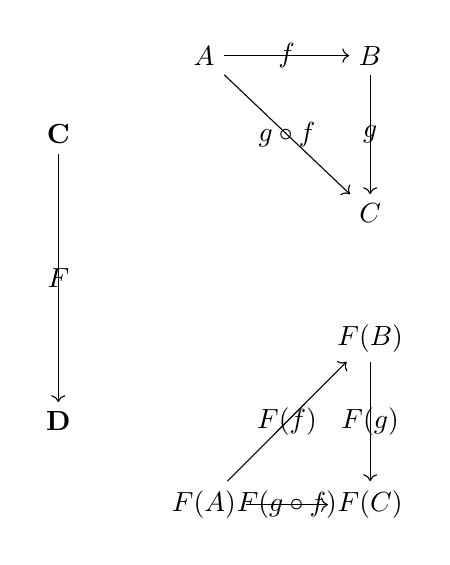
\begin{tikzpicture}
 \matrix (m)[matrix of math nodes,row sep=1.5em,column sep=3em] {
    & A & B \\
  {\bf C} \\
    &   & C \\
  \\
    &   & F(B)\\
  {\bf D} \\
    & F(A) & F(C) \\
 };

 \draw[->] (m-1-2) to node {$f$} (m-1-3);
 \draw[->] (m-1-3) to node {$g$} (m-3-3);
 \draw[->] (m-1-2) to node [swap]{$g \circ f$} (m-3-3);

 \draw[->] (m-2-1) to node [swap]{$F$} (m-6-1);

 \draw[->] (m-7-2) to node {$F(f)$} (m-5-3);
 \draw[->] (m-5-3) to node {$F(g)$} (m-7-3);
 \draw[->] (m-7-2) to node [swap]{$F(g \circ f)$} (m-7-3);
\end{tikzpicture}


ニューラルネットワークの例
\def\layersep{2.5cm}

\begin{tikzpicture}[shorten >=1pt,->,draw=black!50, node distance=\layersep]
    \tikzstyle{every pin edge}=[<-,shorten <=1pt]
    \tikzstyle{neuron}=[circle,fill=black!25,minimum size=17pt,inner sep=0pt]
    \tikzstyle{input neuron}=[neuron, fill=green!50];
    \tikzstyle{output neuron}=[neuron, fill=red!50];
    \tikzstyle{hidden neuron}=[neuron, fill=blue!50];
    \tikzstyle{annot} = [text width=4em, text centered]

    % Draw the input layer nodes
    \foreach \name / \y in {1,...,4}
    % This is the same as writing \foreach \name / \y in {1/1,2/2,3/3,4/4}
        \node[input neuron, pin=left:Input \#\y] (I-\name) at (0,-\y) {};

    % Draw the hidden layer nodes
    \foreach \name / \y in {1,...,5}
        \path[yshift=0.5cm]
            node[hidden neuron] (H-\name) at (\layersep,-\y cm) {};

    % Draw the output layer node
    \node[output neuron,pin={[pin edge={->}]right:Output}, right of=H-3] (O) {};

    % Connect every node in the input layer with every node in the
    % hidden layer.
    \foreach \source in {1,...,4}
        \foreach \dest in {1,...,5}
            \path (I-\source) edge (H-\dest);

    % Connect every node in the hidden layer with the output layer
    \foreach \source in {1,...,5}
        \path (H-\source) edge (O);

    % Annotate the layers
    \node[annot,above of=H-1, node distance=1cm] (hl) {Hidden layer};
    \node[annot,left of=hl] {Input layer};
    \node[annot,right of=hl] {Output layer};
\end{tikzpicture}
% End of code

\end{rem}
\begin{prop}
$\tilde{\sigma} \in Frob(L^{ur}/K) $の不変体を$\Sigma$とする.
$\Sigma$には以下の性質が成り立つ.
 \begin{enumerate}
   \item $\tilde{\sigma}|_{K^{ur}}= \phi_{K^{ur}}^n$とすると,$f_{\Sigma/K}=n$
   \item $[\Sigma:K] < \infty$
   \item $\Sigma^{ur}=L^{ur}$
   \item $\tilde{\sigma}=\phi_{\Sigma}$
 \end{enumerate}
\end{prop}
\begin{proof}
(1)は$\tilde{\sigma}|_{K^{ur}}= \phi_{K^{ur}}^n$より,$\Sigma/K$での剰余体の拡大次数は$n$になるので成り立つ.\\
(2)は$L/K$が有限次拡大なので,惰性群が有限群で$f_{\Sigma/K}$が有限なことより,従う. \\
(3)$\mathrm{Gal}(L^{ur}/\Sigma)$は$\tilde{\sigma}$の一元生成で,$\Sigma/K$が有限次拡大より,無限群になる.無限巡回群の部分群は無限群なので,,$\mathrm{Gal}(L^{ur}/K^{ur}) \cap \langle \tilde{\sigma} \rangle =\{ id \}$となる.よって$L^{ur}/\Sigma$は不分岐拡大. \\
(4)は$L^{ur}/\Sigma$は不分岐拡大なので成り立つ.
\end{proof}
上の結果を元に
$r_{L^{ur}/K}Frob(L^{ur}/K) \to K^{\times}/N_{L^{ur}/K}{L^{ur}}^{\times}$を定義する.
ただし,$N_{L^{ul}/K}{L^{ur}}^{\times}$は$\displaystyle \bigcap_{M,[M:K]< \infty}N_{M/K}(M^{\times})$で定める.
\begin{lem}
$\pi_{\Sigma}$を$\Sigma$の素元とする.
 \begin{equation*}
  r_{L^{ur}/K}(\sigma)=N_{\Sigma/K}(\pi_{\Sigma})\ \mbox{mod}\ N_{L^{ur}/K}{L^{ur}}^{\times}
 \end{equation*}
は$\pi_{\Sigma},\tilde{\sigma}$のとり方によらない.
\end{lem}
\begin{proof}
$\Sigma$の素元は$u \in U_{\Sigma}$を用いて,$u \pi_{\Sigma}$と書けるので,
$N_{\Sigma/K}(u) \in N_{L^{ur}/K}L^{\times}$を示せれば良い.
つまり,$L^{ur}/K$の有限次部分体$M$に対し,$N_{\Sigma/K}(u) \in N_{M/K}(M^{\times})$
が示せればよい.$K$の有限次拡大体$M_1\subset M_2$に対し.$N_{M_1/K}(M_1^{\times}) \supset N_{M_2/K}(M_2^{\times})$となるので,$\Sigma \subset M$の場合にのみ示せばよい.(そうでない場合は$\Sigma$との合成体について示せば上に記した性質より言える.)
$\Sigma^{ur}=L^{ur}$より$M/\Sigma$は不分岐拡大で,$N_{M/\Sigma}(U_M)=U_{\Sigma}$となるので,従う.
$\tilde{\sigma}$によらないことを示す.$\tilde{\sigma_1},\tilde{\sigma_2} \in Frob(L^{ur}/K)$で,$\tilde{\sigma_1}|_L=\tilde{\sigma_2}|_L=\sigma$とする.
この時,$\pi_{\Sigma_1},\pi_{\Sigma_2}$は$L^{ur}$の素元になるので,
$N_{\Sigma_1/K}(\pi_{\Sigma_1})=N_{\Sigma_1/\Sigma_1\cap K^{ur}} \circ N_{\Sigma_1\cap K^{ur}/K}(\pi_{\Sigma_1}) $
となる.
ここで不分岐拡大は拡大次数が定まれば一意に定まることから
$\Sigma_1\cap K^{ur}/K = \Sigma_2\cap K^{ur}/K$となり,$\Sigma_1^{ur}=L^{ur}=\Sigma_2^{ur}$より,
$\mathrm{Gal}(L^{ur}/K^{ur}) \simeq \mathrm{Gal}(\Sigma_1/\Sigma_1 \cap K^{ur}) \simeq \mathrm{Gal}(\Sigma_2/\Sigma_2 \cap K^{ur})$となる.
これより,$N_{\Sigma_1/K}(\pi_{\Sigma_1}) \cdot {N_{\Sigma_2/K}(\pi_{\Sigma_2})}^{-1}$は$\pi_{\Sigma_1},\pi_{\Sigma_2}$は$\Sigma_1 \Sigma_2$の素元になるので,$\pi_{\Sigma_1},\pi_{\Sigma_2}$をうまくとるととも$\Sigma_1  \cap \Sigma_2$
の元にできるので,$N_{\Sigma_1/K}(\pi_{\Sigma_1}) \cdot {N_{\Sigma_2/K}(\pi_{\Sigma_2})}^{-1}= N_{\Sigma_1 \cap \Sigma_2}/K u$
とかける.不分岐拡大では単元全体から単元全体への写像は全射となるので,上の元は任意の体からのノルムの元として存在する.
よって体のとり方によらない.
\end{proof}

$L/K$が無限次元代数拡大の時,以下でノルムを定める.
\begin{equation*}
  N_{L/K}(L^{\times}):=\bigcap_{[M:K] < \infty} N_{M/K}M^{\times}
\end{equation*}

\begin{prop}
 \begin{equation*}
  r_{L^{ur}/K}:Frob( L^{ur}/K ) \to K^{\times}/N_{L^{ur}/K}{L^{ur}}^{\times}
 \end{equation*}
 は乗法的である.
\end{prop}
\begin{proof}
$r_{L^{ur}/K} (\sigma_1 \cdot  \sigma_2) = r_{L^{ur}/K}(\sigma_1) \cdot r_{ L^{ur}/K}(\sigma_2)$
を示せば良い.$\sigma_1 \cdot \sigma_2 =\sigma_3$とする.それぞれの不変体を$\Sigma_1,\Sigma_2,\Sigma_3$とすると,
$\Sigma_1 \Sigma_2 \Sigma_3$は$\sigma_1,\Sigma_2,\Sigma_3$の不分岐拡大体となる.
今$\phi \in Frob(L^{ur}/K)$を$\phi|_{K^{ur}}$がFrobeniusとなるものとする.
この時,$N_{\Sigma_1/K}(\pi_{\Sigma_1}) = N_{L^{ur}/K^{ur}} (\pi_{\Sigma_1}^{\frac{\phi^{n_1}-1}{\phi -1}}) $
となる.
同様に計算すると
\begin{equation*}
  N_{\Sigma_1/K}(\pi_{\Sigma_1})  \cdot N_{\Sigma_2/K}(\pi_{\Sigma_2})  {N_{\Sigma_3/K}(\pi_{\Sigma_3})}^{-1} =
  N_{L^{ur}/K^{ur}} (\pi_{\Sigma_1}^{\frac{\phi^{n_1}-1}{\phi -1}})  \cdot N_{L^{ur}/K^{ur}} (\pi_{\Sigma_2}^{\frac{\phi^{n_2}-1}{\phi -1}})
  (N_{L^{ur}/K^{ur}} (\pi_{\Sigma_3}^{\frac{\phi^{n_3}-1}{\phi -1}}))^{-1}
\end{equation*}
となり,$n_1 + n_2 = n_3$より,計算すれば,ある$u \in \Sigma_1 \Sigma_2 \Sigma_3$が存在し,$N_{L^{ur}/K^{ur}}u$とかけることがわかる.
これと不分岐拡大の単元の全射性より,$N_{L^{ur}/K^{ur}}u \in N_{L^{ur}/K} {L^{ur}}^{\times}$となる.
よって示された.
\end{proof}

これから,以下が成り立つ
\begin{cor}
 $L/K$を局所体の有限次ガロア拡大とすると相互写像
 \begin{equation*}
  r_{L/K}: \mathrm{Gal}(L/K) \to K^{\times}/N_{L/K}L^{\times}
 \end{equation*}
 は準同型になる.
\end{cor}

\begin{cor}
 $L/K$が局所体の有限次不分岐拡大とする.相互写像は同型写像となる.
\end{cor}
\begin{proof}
 $N_{L/K}U_L=U_K$となり,付値を計算すると,位数は同じ巡回群となる.
 また$L/K$のFrobeniusの不変体は$L$となり,$N_{L/K}\pi_L$は位数が$[L:K]$の元となるので,
 生成元が生成元へと移る.
\end{proof}


局所相互写像が同型であることをしめす.


\begin{thm}
 局所体の任意の有限次ガロア拡大$L/K$に対し,相互写像は同型写像である.
\end{thm}
\begin{proof}
$ _{N_{L/K}}L^{\times} = I_G L^{\times}$と$\# K^{\times}/N_{L/K}L^{\times} =[L:K]$を用いて同型写像であることを示す.
$L/K$が有限次巡回完全分岐拡大の場合に示せば良いことを示す.
******************\\
あとで埋める \\
******************\\
完全分岐巡回拡大の時は
$\# K^{\times}/N_{L/K}L^{\times} =[L:K]$から,$r_{L/K}$が単射であることを示せば良い.
$\sigma \in \mathrm{Gal}(L/K)$の生成元とし,$\Sigma$を$L^{ur}/K$での$\overline{\sigma}$の不変体とする.
$\Sigma L/L,\Sigma L/\Sigma$は不分岐拡大なので,
$\pi_{\Sigma}$と$\pi_L$は$\Sigma L$の合成体の素元となる.
よって,ある$u \in \Sigma L$が存在し,$\pi_{\Sigma}^k = u \pi_L^k$とかける.
また,$\mathrm{Gal}(L^{ur}/K^{ur}) \simeq \mathrm{Gal}(L/K) \simeq \mathrm{Gal}(\Sigma/K)$なので,
\begin{equation*}
 r_{L/K}(\sigma^k) \equiv N_{L^{ur}/K^{ur}}(\pi_{\Sigma}^k) \equiv N_{L^{ur}/K^{ur}}(u) \quad \mbox{mod} N_{L^{ur}/K^{ur}}L^{\times}
\end{equation*}
今$r_{L/K}(\sigma^k)=1$とすると$N_{L^{ur}/K^{ur}}(uv^{-1})=1$となる$v \in U_L$が存在する.
$M$を$\Sigma L/K$の最大不分岐拡大とすると.ある$a \in \Sigma L$が存在し,$ a^{\sigma -1}= uv^{-1}$となる.
これより,
$x=\pi_L^kva^{1-\tilde{\sigma}}$が$M^{\times}$の元となることを示す.すると
$v_M$を$M$の正規付値とすると$nv_M(x)=k$となるので,$k$は$n$で割り切れ,特に単射であることが従う.
そのためには$x^{\tilde{\sigma} -1} =1$であることを示せばよい.
\begin{equation*}
(\pi_L^kv)^{\sigma -1}= (\pi_{\Sigma}^ku^{-1}v)^{\tilde{\sigma}-1} =(a^{\sigma -1})^{\tilde{\sigma}-1}
\end{equation*}
より,従う.
\end{proof}


- 局所体の相互写像
- 局所類体論の証明
- $\mathbb{Q}_p$の最大アーベル拡大体の決定
- Lubin-Tate拡大
大域類体論へ

\section{アデールとイデール}
\label{sec:アデールとイデール}
定義
類体公理の確認
分岐?

\section{大域類体論の応用}
\label{sec:大域類体論の応用}
- 冪剰余の相互法則
- Artin L関数とHecke L関数
- Poitou-Tate exact sequence
- 岩澤理論の基本完全系列

\end{document}
